\documentclass{latex-template/tufte-handout}

\title{Introduction to Python Programming Installation Guide}

\setcounter{secnumdepth}{2}

%\author[The Tufte-LaTeX Developers]{The Tufte-\LaTeX\ Developers}

\date{2022-2023} % without \date command, current date is supplied

%\geometry{showframe} % display margins for debugging page layout

\usepackage{graphicx} % allow embedded images
  \setkeys{Gin}{width=\linewidth,totalheight=\textheight,keepaspectratio}
  \graphicspath{{graphics/}} % set of paths to search for images
\usepackage{amsmath}  % extended mathematics
\usepackage{booktabs} % book-quality tables
\usepackage{units}    % non-stacked fractions and better unit spacing
\usepackage{multicol} % multiple column layout facilities
\usepackage{lipsum}   % filler text
\usepackage{fancyvrb} % extended verbatim environments
  \fvset{fontsize=\normalsize}% default font size for fancy-verbatim environments
\usepackage{cleveref}

% Standardize command font styles and environments
\newcommand{\doccmd}[1]{\texttt{\textbackslash#1}}% command name -- adds backslash automatically
\newcommand{\docopt}[1]{\ensuremath{\langle}\textrm{\textit{#1}}\ensuremath{\rangle}}% optional command argument
\newcommand{\docarg}[1]{\textrm{\textit{#1}}}% (required) command argument
\newcommand{\docenv}[1]{\textsf{#1}}% environment name
\newcommand{\docpkg}[1]{\texttt{#1}}% package name
\newcommand{\doccls}[1]{\texttt{#1}}% document class name
\newcommand{\docclsopt}[1]{\texttt{#1}}% document class option name
\newenvironment{docspec}{\begin{quote}\noindent}{\end{quote}}% command specification environment

\hypersetup{colorlinks}

\begin{document}

\maketitle% this prints the handout title, author, and date

\begin{abstract}
\noindent
This guide explains how to install the required tools (Python, Jupyter, and Anaconda) for the course.
Moreover, this guide also shows how to use Jupyter notebooks within VS Code.

\end{abstract}




\section{Introduction} \label{introduction}
%\begin{fullwidth}



In this course we will be using \href{https://www.python.org}{\textbf{Python 3}} as programming language. In addition, all the tools that we will require along the course are part of the \href{https://anaconda.org}{\textbf{Anaconda}} distribution. 
Anaconda is a distribution of Python and R, and it is mostly used for data science tasks. It also eases package management and deployment processes. The distribution is available for \emph{Windows}, \emph{Linux}, and \emph{MacOS}.
\begin{marginfigure}%
  
\includegraphics[width=\linewidth]{assets/python-logo}
  \label{fig:marginfig}
\end{marginfigure}

Moreover, Anaconda comes with the \textbf{Anaconda Navigator}, which is
a Graphical User Interface (GUI) that includes a set of tools such as:
\begin{marginfigure}%
  
\includegraphics[width=\linewidth]{assets/anaconda-logo}
  \label{fig:marginfig}
\end{marginfigure}

\begin{quote}
\begin{enumerate}
%\def\labelenumi{\arabic{enumi}.}
\item
  \href{https://jupyter.org}{\textbf{Jupyter} (\textbf{Notebook} and
  \textbf{JupyterLab})}: web platforms that support the interaction with
  computational notebooks. For the course, you can use either of them.
\item
  \href{https://www.spyder-ide.org}{\textbf{Spyder}} and
  \href{https://www.jetbrains.com/pycharm/}{\textbf{PyCharm}}:
  Integrated Development Environments (IDEs) to interact with Python
  scripts and projects.
\item
  \href{https://docs.conda.io/en/latest/}{\textbf{Conda}}:
  language-agnostic package manager.
\end{enumerate}
\end{quote}

%\end{fullwidth}

\begin{center}\rule{\linewidth}{0.5pt}\end{center}

\section{Required Tools}

Use the installer for \textbf{Anaconda3 2021-05} with \textbf{Python
3.8}.% Details are given below. You can install \textbf{Anaconda3 2021-05} wich works with \textbf{Python 3.8} but you might find inconsistencies.\\
Installers are available for \textbf{Windows}, \textbf{MacOS}, \textbf{Linux}.\\

\begin{center}\rule{\linewidth}{0.5pt}\end{center}


\subsection{Download Anaconda Installer}\label{download-anaconda-installer}

Download the Individual Edition of Anaconda. Choose the Python 3.8
version installer for your platform \href{https://repo.anaconda.com/archive/}{here}.

If you have trouble downloading or finding the specific installer, you
can download yours from the following links:
\begin{quote}
	
\begin{itemize}
\item \href{https://repo.anaconda.com/archive/Anaconda3-2021.05-Windows-x86.exe}{Windows
  32-bit}\\
\item \href{https://repo.anaconda.com/archive/Anaconda3-2021.05-Windows-x86_64.exe}{Windows
  64-bit}\\
\item \href{https://repo.anaconda.com/archive/Anaconda3-2021.05-MacOSX-x86_64.pkg}{MacOS}\\
\item \href{https://repo.anaconda.com/archive/Anaconda3-2021.05-Linux-x86_64.sh}{Linux
  (x86)}\\
\item \href{https://repo.anaconda.com/archive/Anaconda3-2021.05-Linux-ppc64le.sh}{Linux
  (Power8 and Power9)}
\end{itemize}
\end{quote}

See \Cref{notes-on-updating} at the end of these instructions.
% TODO fix ref

\subsection{Install Anaconda}\label{install-anaconda}

Follow the installation guidelines for your platform:

\begin{quote}
\begin{itemize}
\item \href{https://docs.anaconda.com/anaconda/install/windows/}{Windows}\\
\item \href{https://docs.anaconda.com/anaconda/install/mac-os/}{MacOS}
\item \href{https://docs.anaconda.com/anaconda/install/linux/}{Linux}\\
\item \href{https://docs.anaconda.com/anaconda/install/linux-power8/}{Linux (Power)}
\item \href{https://docs.anaconda.com/anaconda/install/}{Other platforms}.
\end{itemize}
\end{quote}


\section{Create Virtual Environment}
Anaconda allows us to create \emph{virtual environments} easily.
A virtual environment is an isolated, working copy of Python with its files, directories, and libraries so that you can work with specific versions of libraries without affecting other Python projects or installations.

To create a new virtual environment, please follow the next steps:


\begin{quote}
	\begin{enumerate}
		\item Launch the Anaconda navigator.
			\begin{marginfigure}[-50em]
			  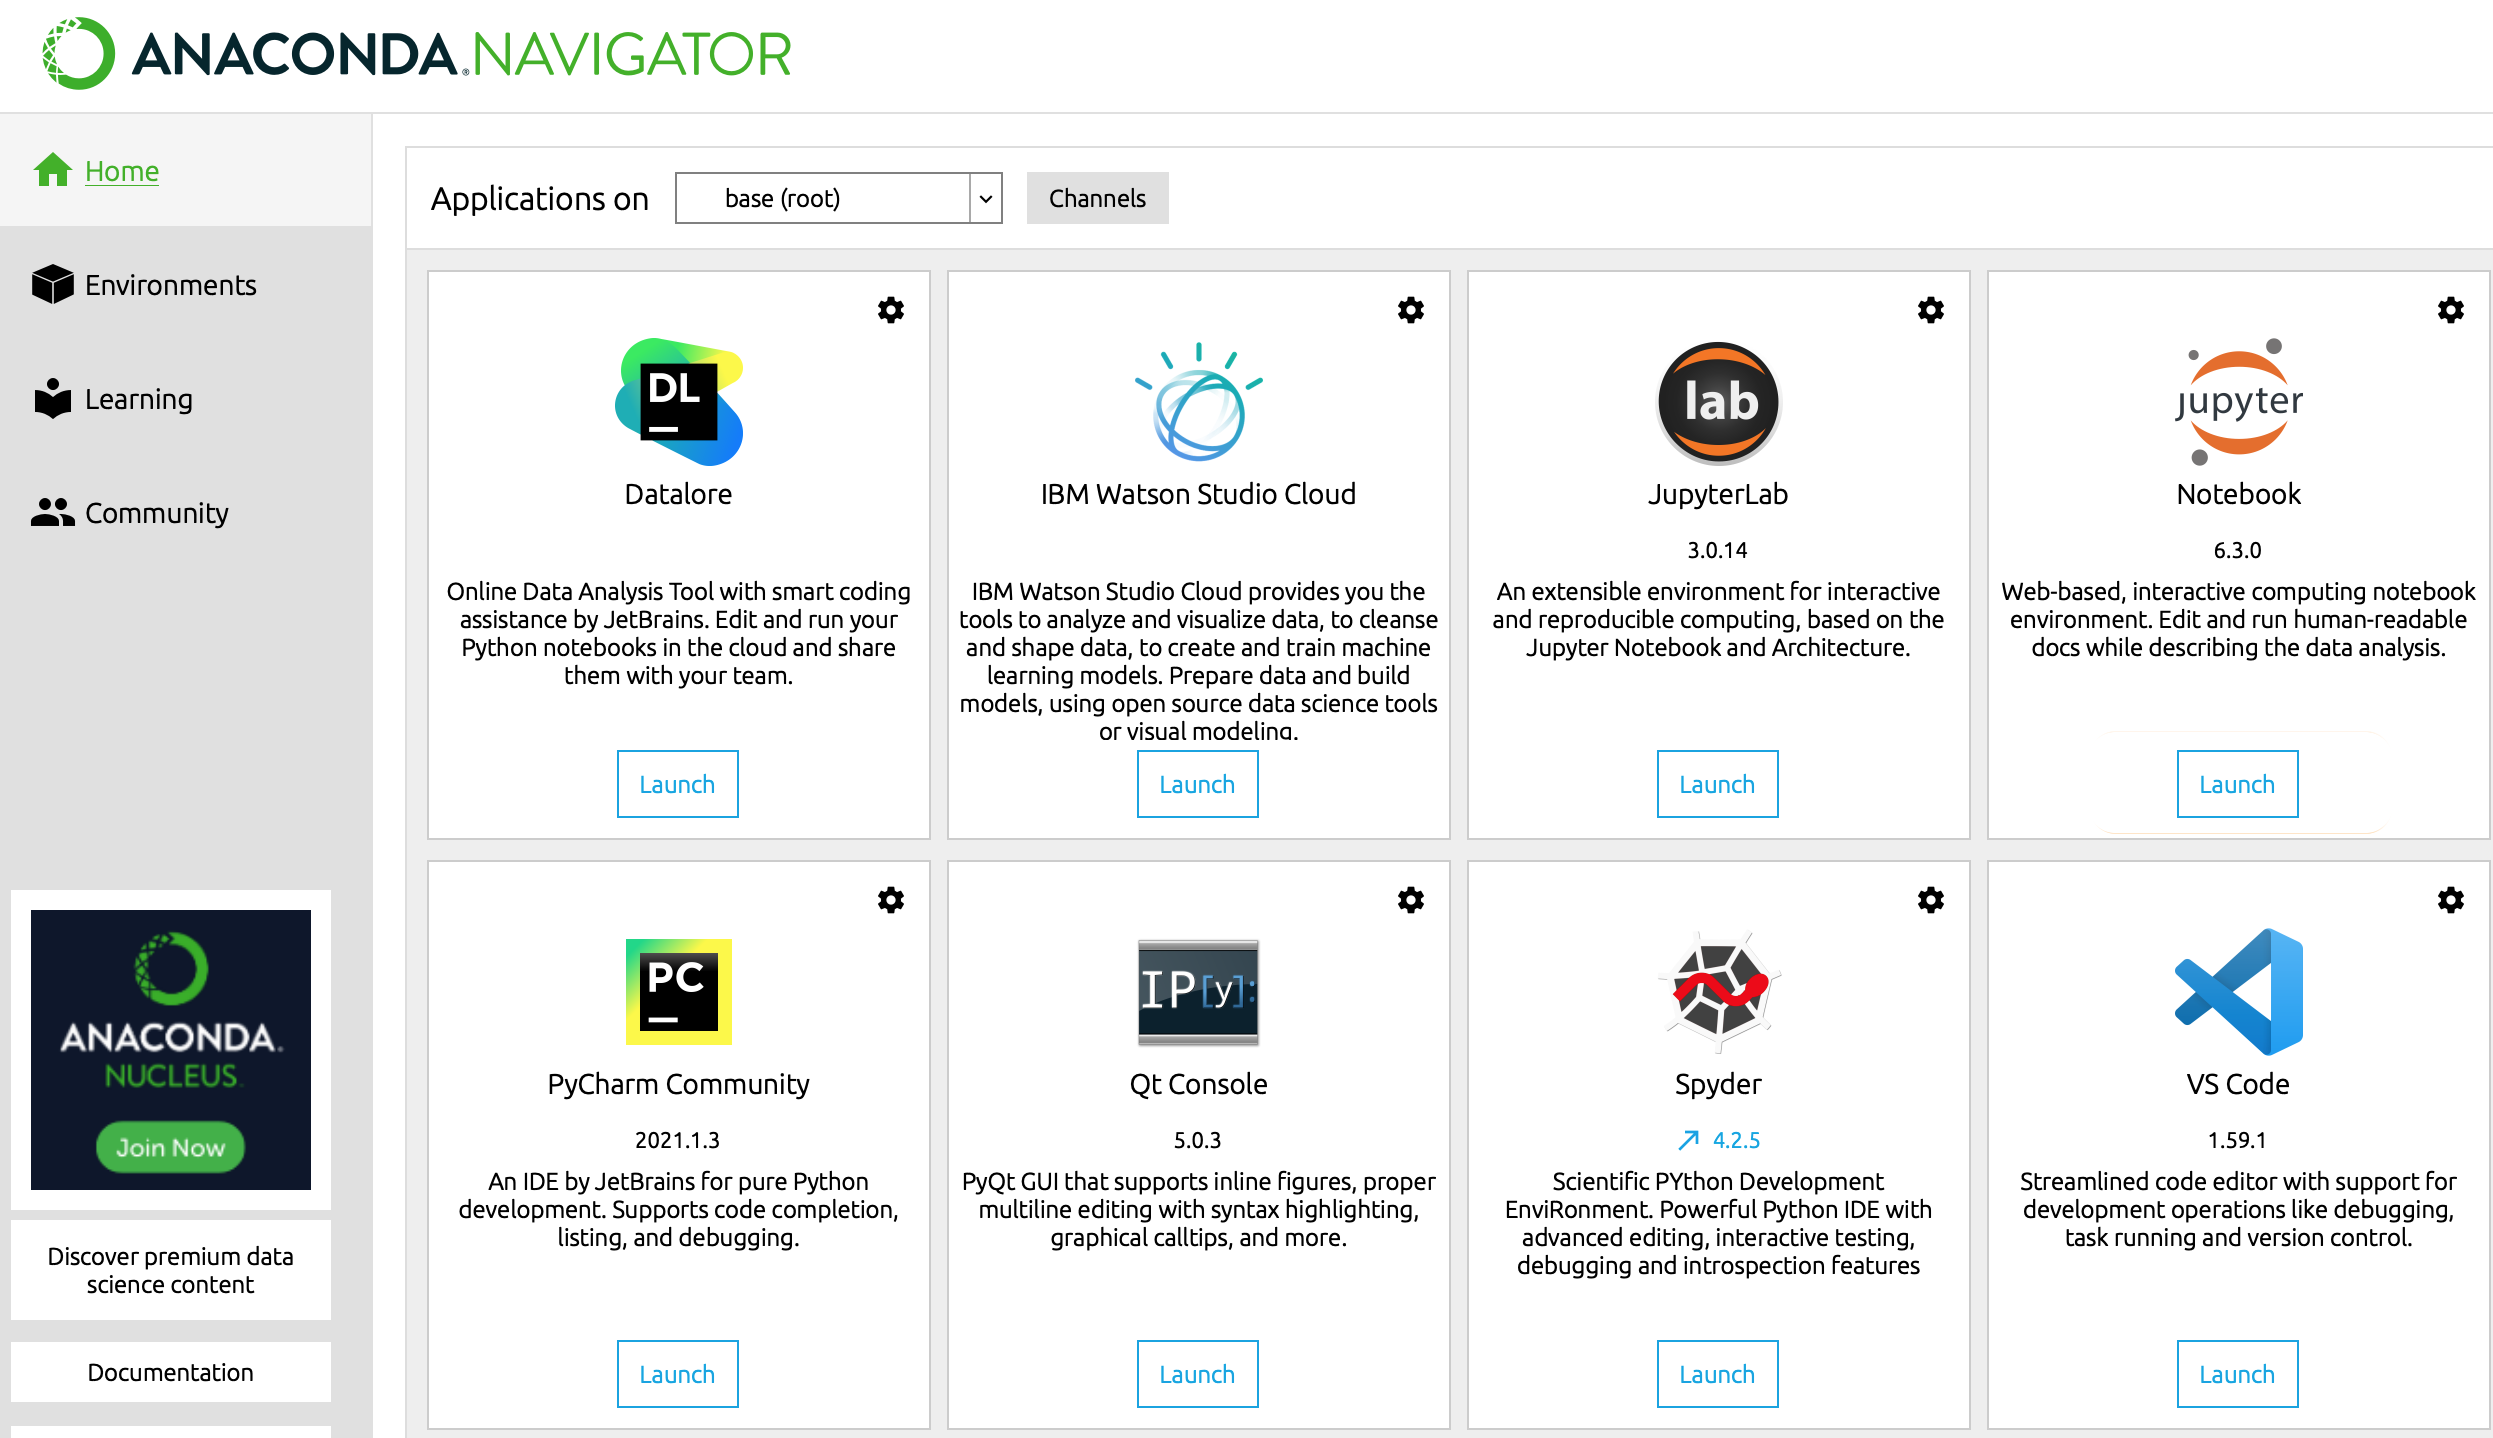
\includegraphics[width=1.2\linewidth]{assets/01-launch}
			  \caption{Anaconda navigator.}
			  \label{fig:img1}
			\end{marginfigure}
			\begin{marginfigure}[-28em]%
			  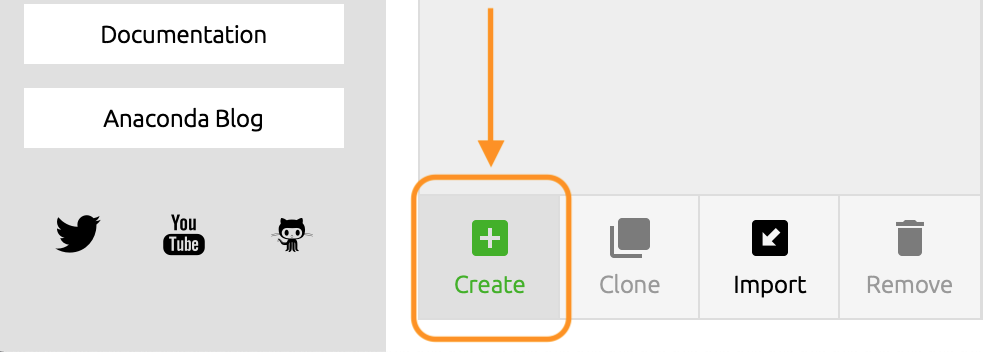
\includegraphics[width=\linewidth]{assets/02-create-ve}
			  \caption{Create virtual environment.}
			  \label{fig:img2}
			\end{marginfigure}
		\item Click on \emph{Environments} (top left pane of the window), and then click on the \emph{create} button (bottom left part of the screen) (see \Cref{fig:img2}).
		\item Then, you can assign a name to the new virtual environment (e.g., JBI010) and choose the correct Python version. During the course, we will work with Python 3.8 (see \Cref{fig:img3}).
			\begin{marginfigure}[-20em]%
			  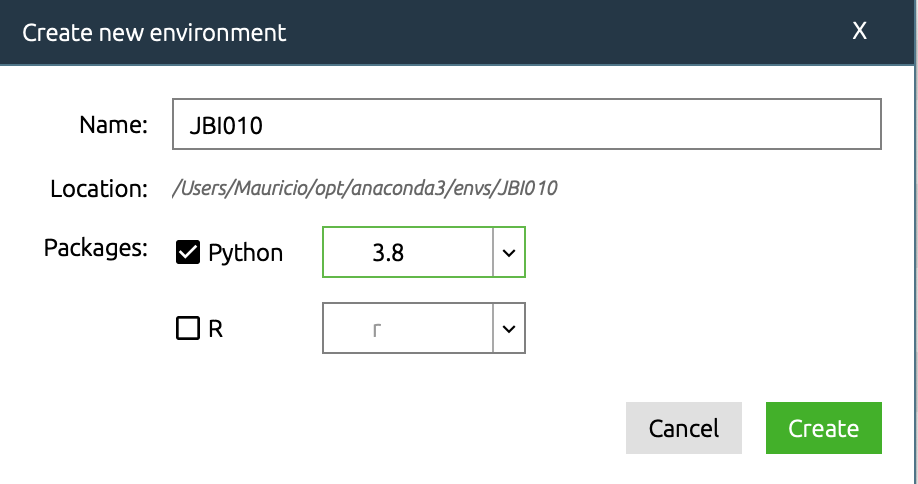
\includegraphics[width=\linewidth]{assets/03-python-version}
			  \caption{Choose Python version.}
			  \label{fig:img3}
			\end{marginfigure}
		\item Now we will select the virtual environment we want to use. To do so, click on the \emph{Home} button (left pane of the Anaconda navigator) and click on the dropdown list next to the channels button (see \Cref{fig:img4}).
			\begin{marginfigure}[-7em]%
			  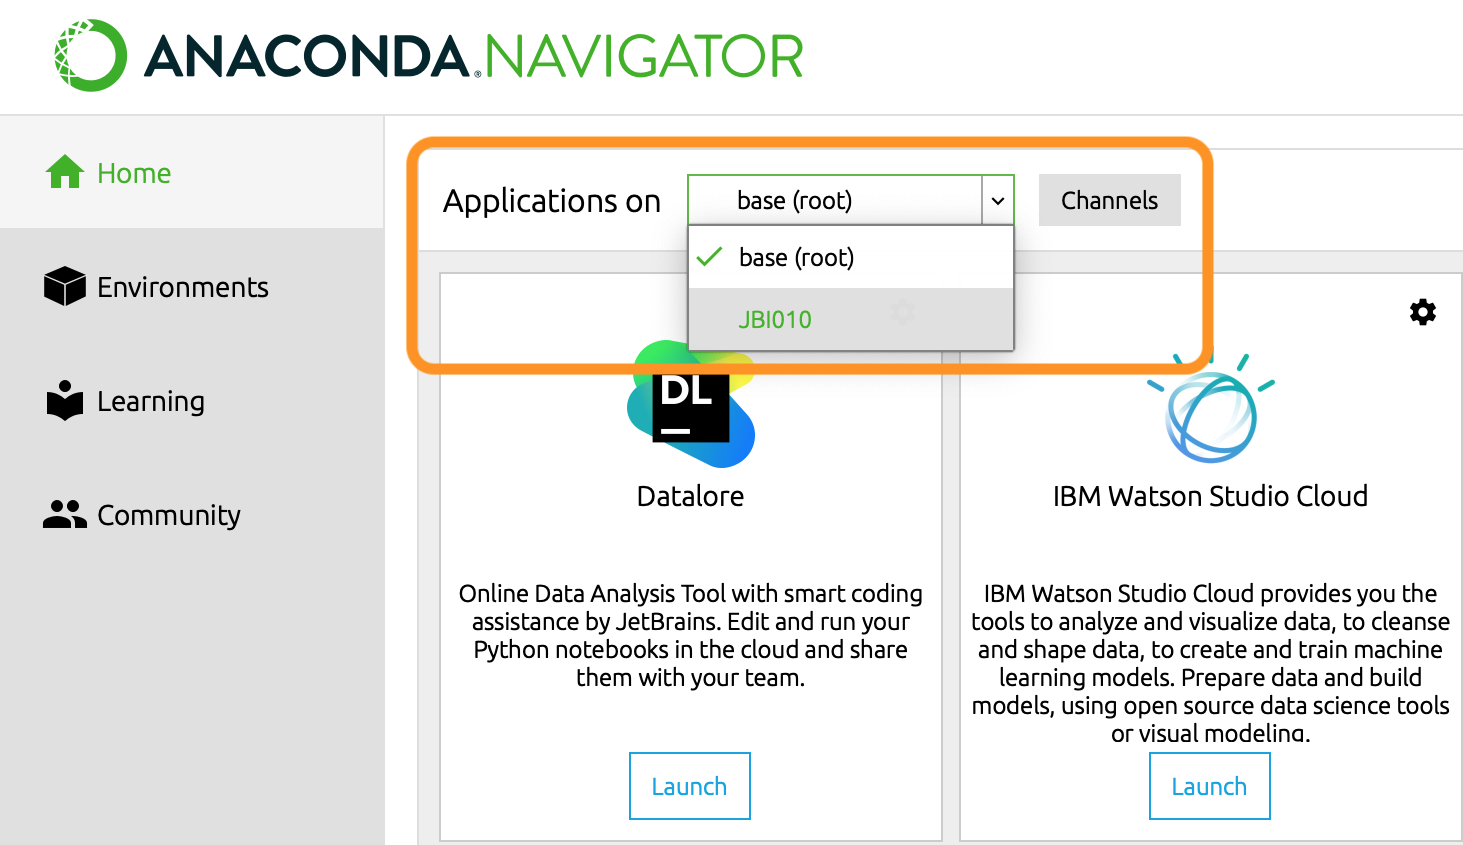
\includegraphics[width=\linewidth]{assets/04-choose-ve}
			  \caption{Choose the virtual environment created in the previous step.}
			  \label{fig:img4}
			\end{marginfigure}
		\item To install Jupyter, you have to  look for the Jupyter logo and click on the \emph{install button} (see \Cref{fig:img5}). This process might take some minutes.
			\begin{marginfigure}%
			  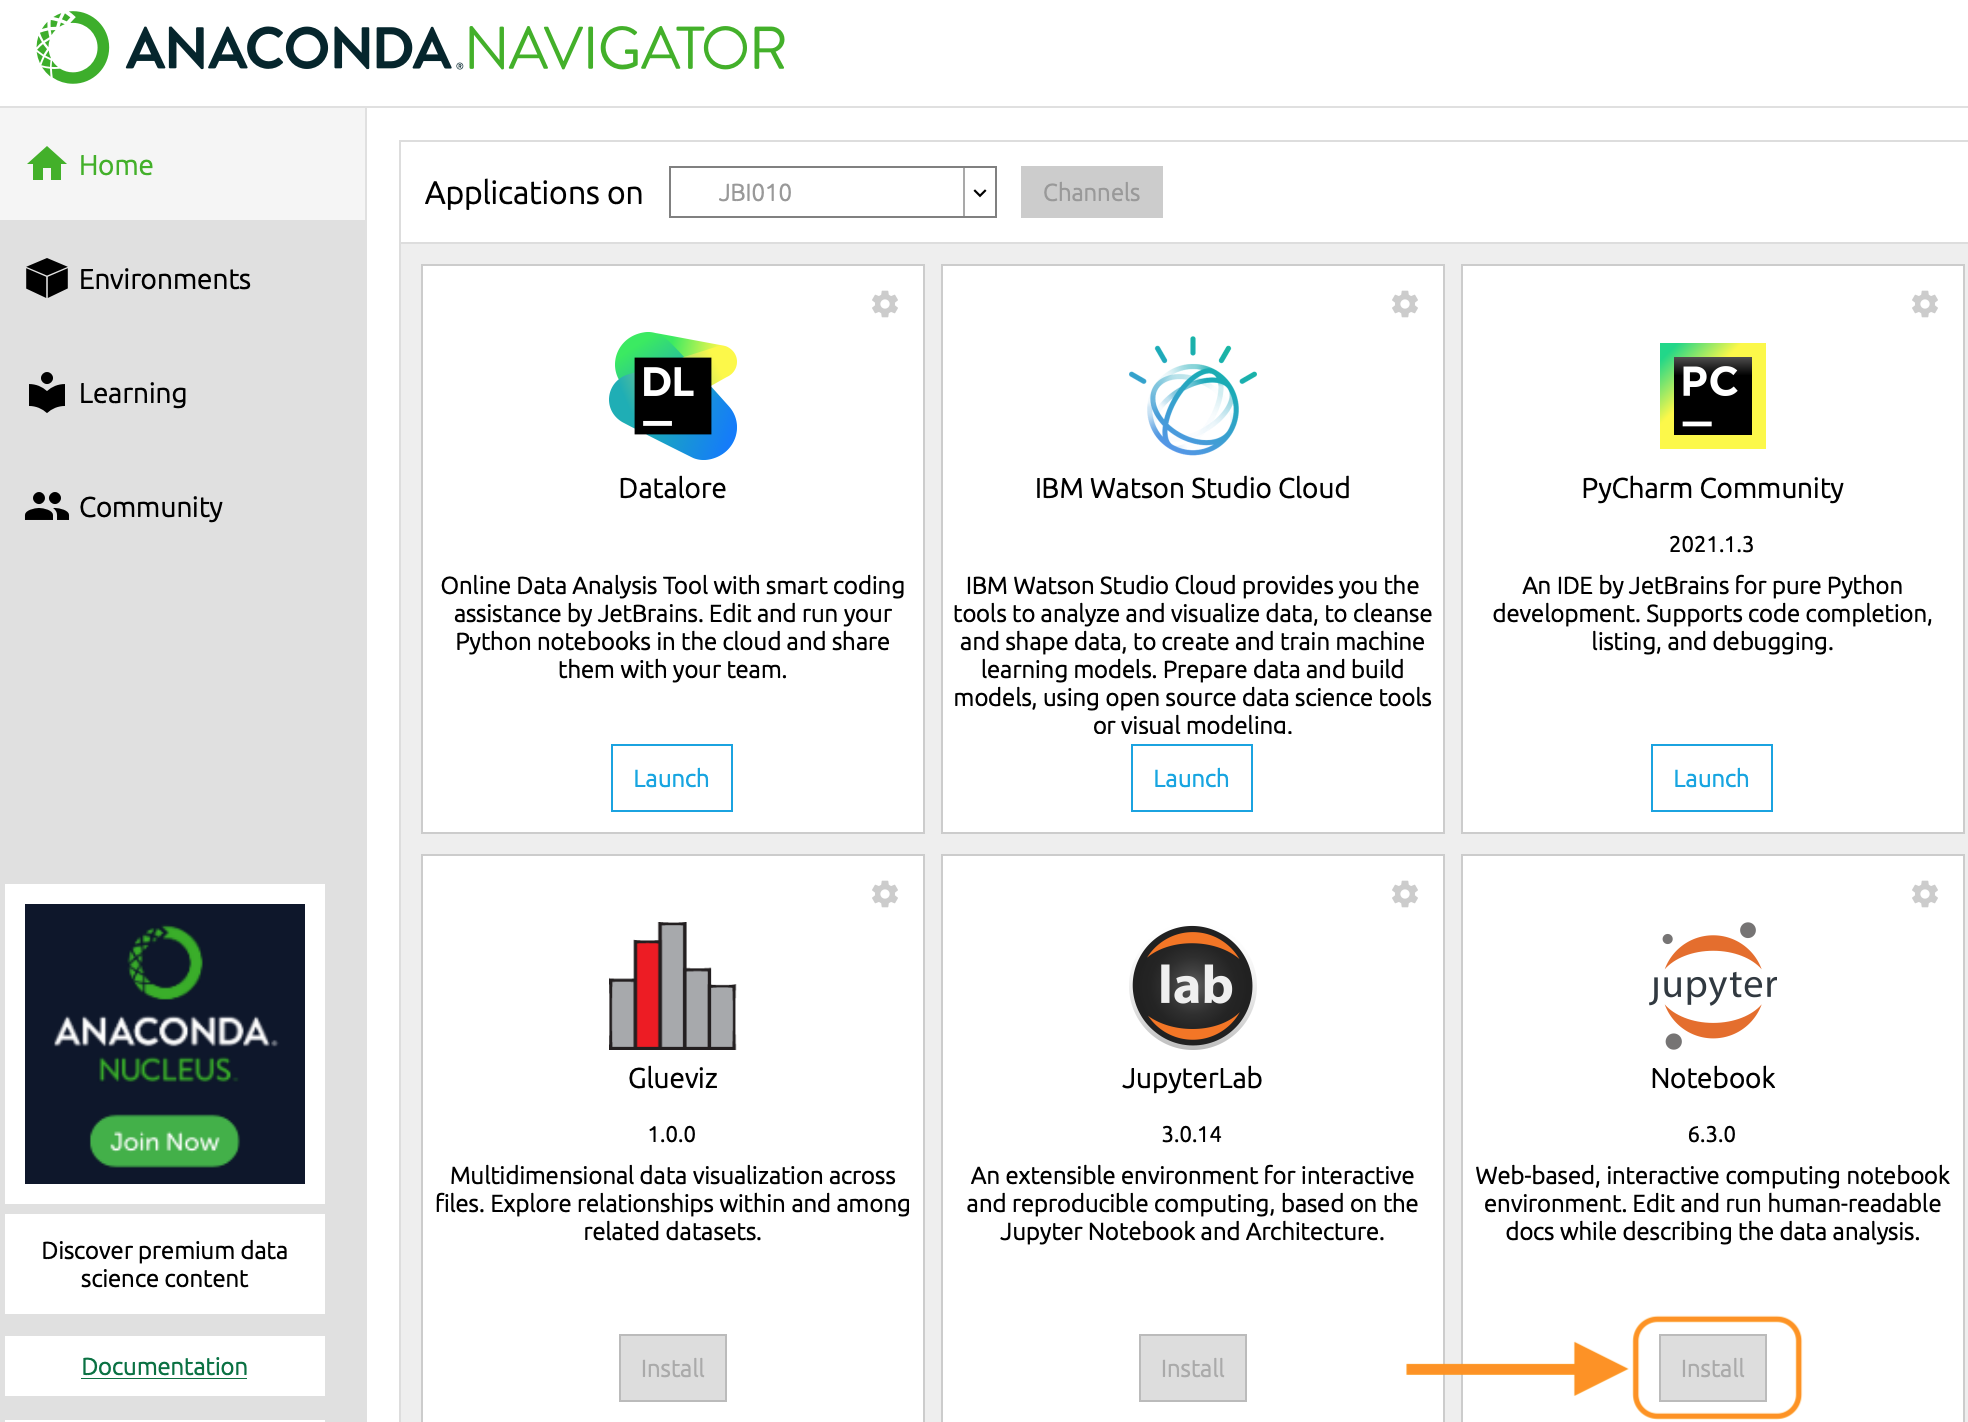
\includegraphics[width=1.2\linewidth]{assets/05-install-jupyter}
			  \caption{Installing Jupyter notebook.}
			  \label{fig:img5}
			\end{marginfigure}
	\end{enumerate}
\end{quote}



\section{Verify Tools Installation}\label{verify-tools-installation}

After installing the tools, you should verify them. To do so:

\begin{quote}
\begin{enumerate}
\def\labelenumi{\arabic{enumi}.}
\item Download from \textbf{\href{https://canvas.tue.nl}{Canvas}} the notebook of the week 0 assignment (i.e.~\href{https://canvas.tue.nl/courses/19301/assignments/69081}{Assignment-0-template.zip}).
\item Launch the Anaconda-Navigator (see \Cref{fig:anaconda-navigator}).
\item In it, select Jupyter Notebook (or JupyterLab if you prefer) and click
  on the \emph{launch} button.
\item Navigate to the downloaded notebook and open it (\Cref{fig:week-0}).
\item Follow the instructions in the notebook.
\item Save the executed notebook: File \textgreater{} Save and Checkpoint.
\end{enumerate}

\end{quote}

\begin{marginfigure}%
  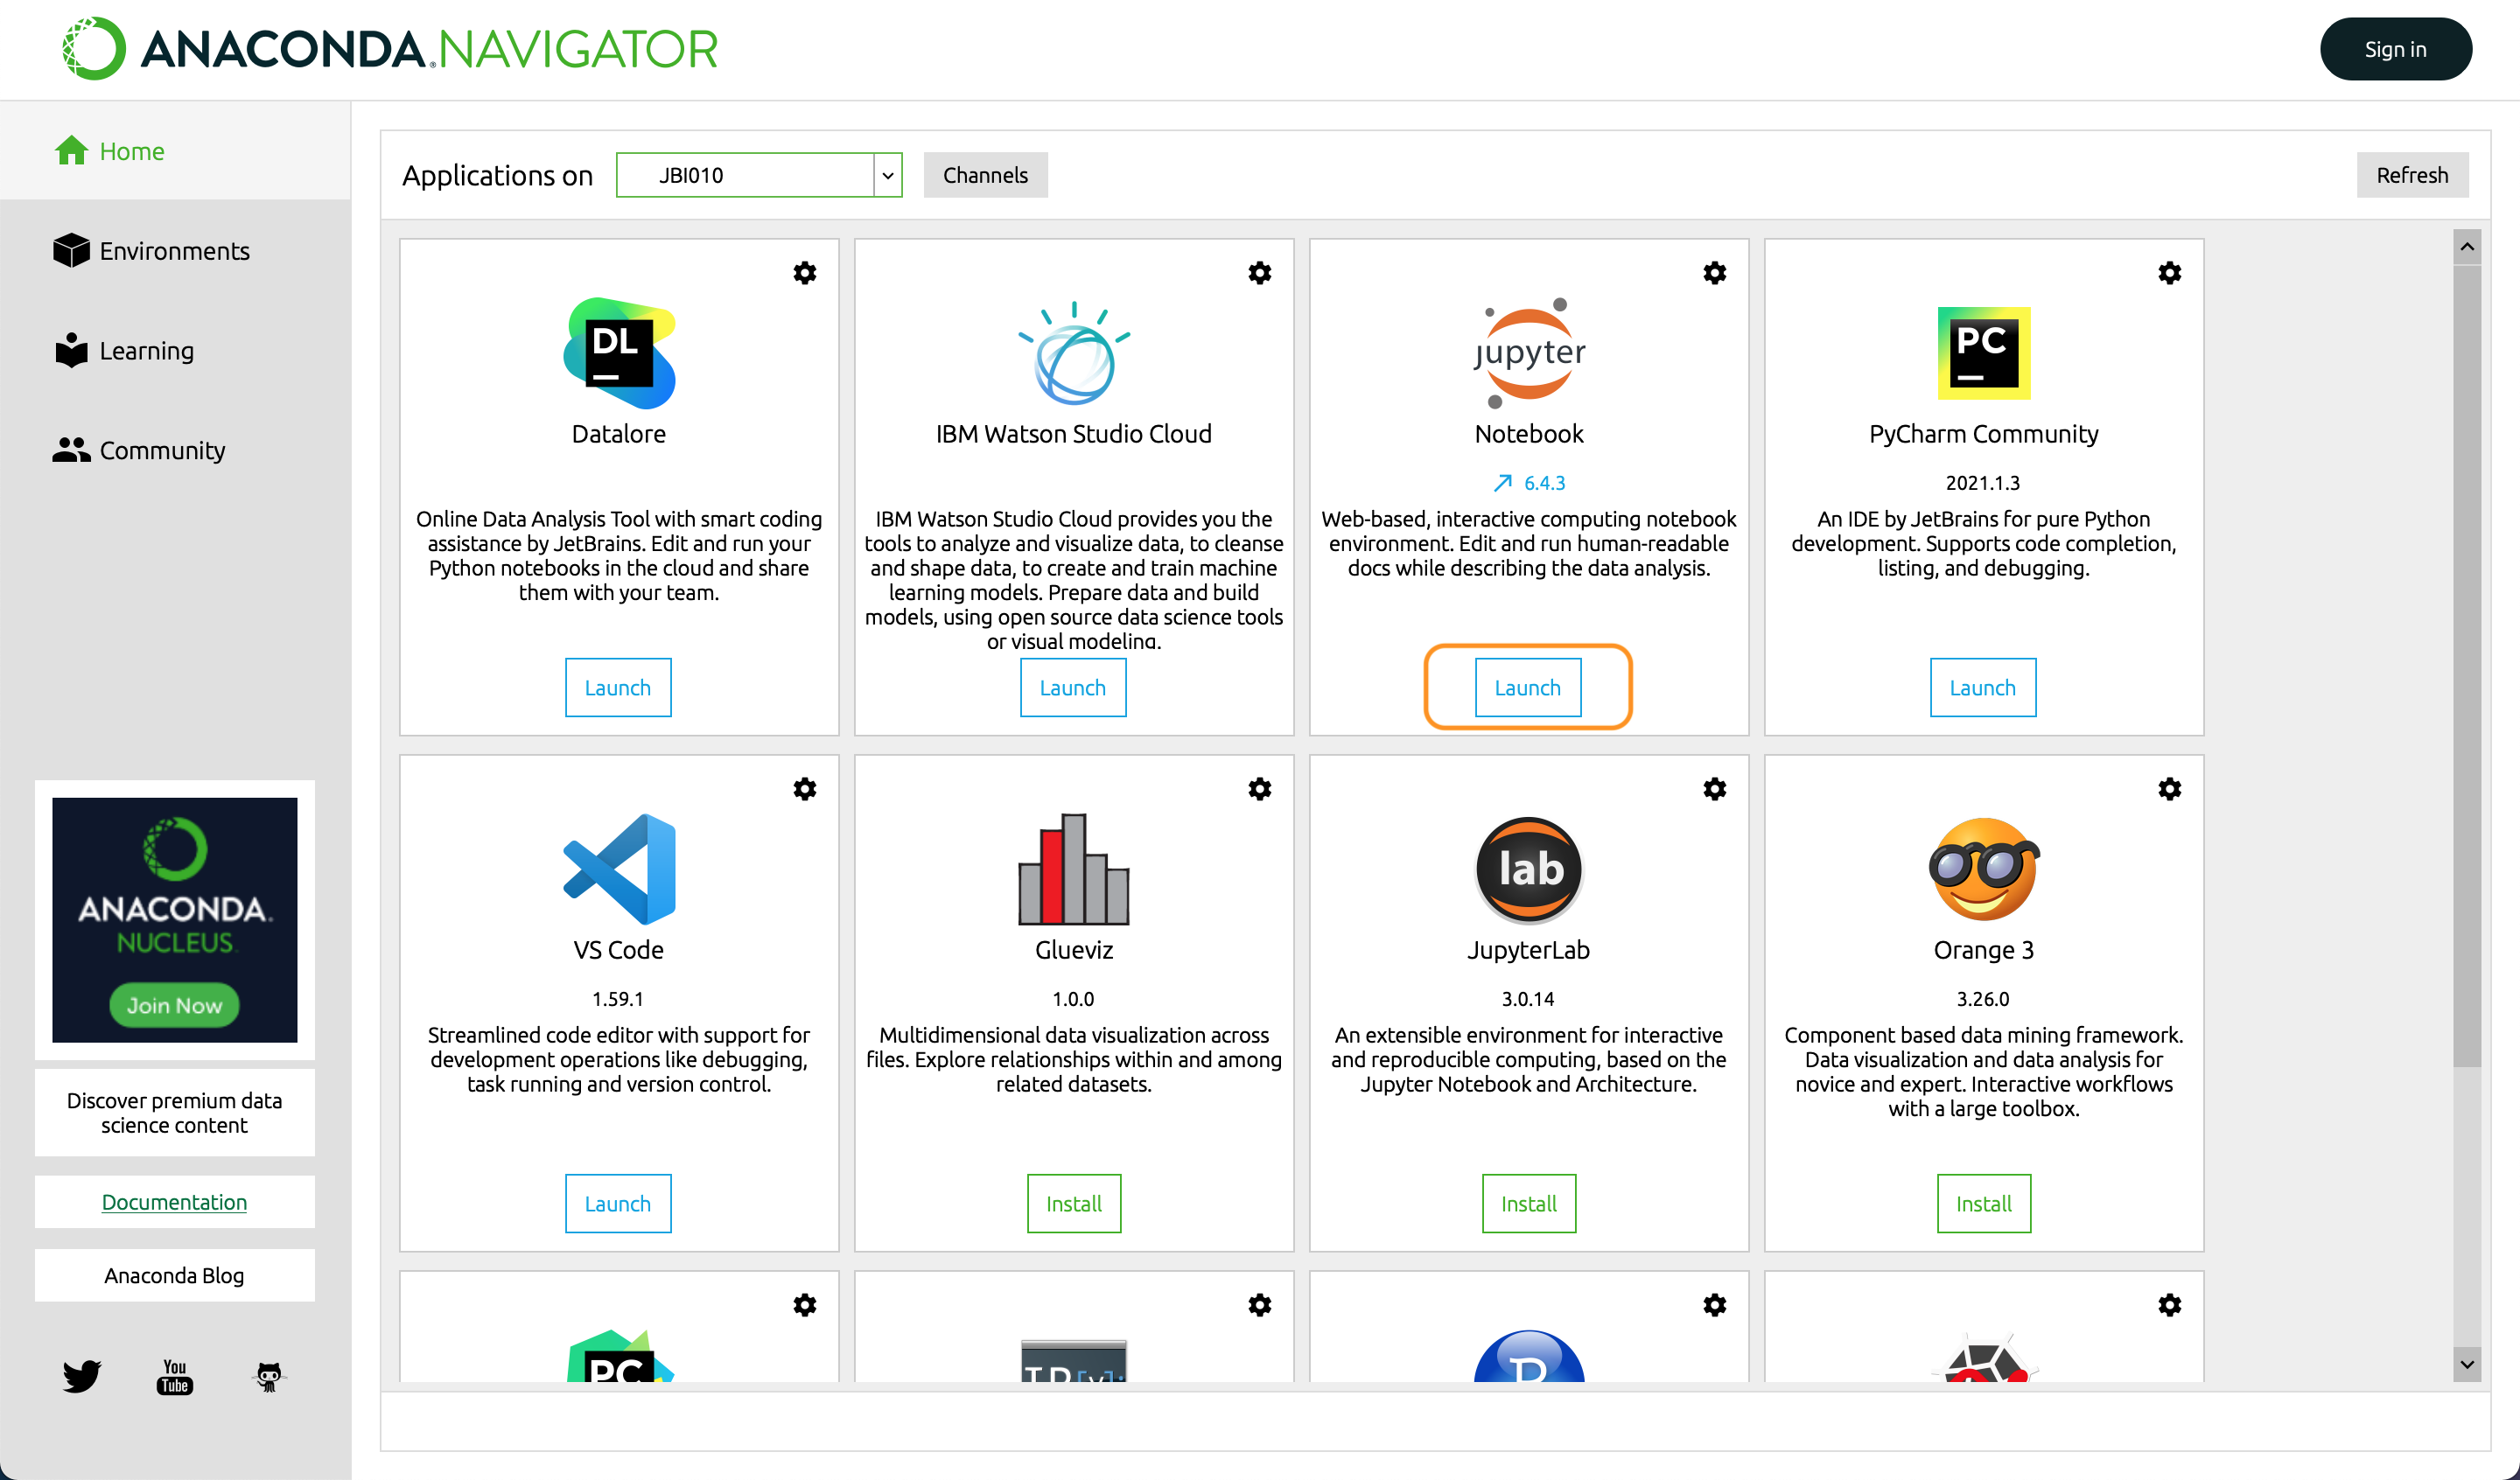
\includegraphics[width=1.3\linewidth]{assets/06-launch-jupyter}
  \caption{Anaconda navigator.}
  \label{fig:anaconda-navigator}
\end{marginfigure}



\begin{marginfigure}%
  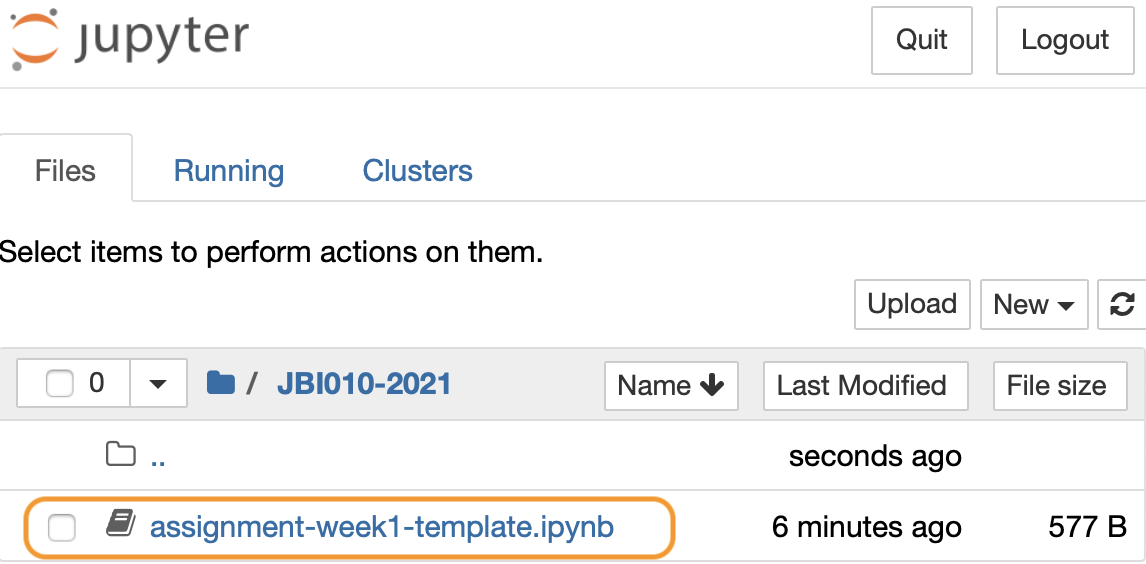
\includegraphics[width=1.2\linewidth]{assets/open-nb}
  \caption{Jupyter notebook of the assignment of week 0.}
  \label{fig:week-0}
\end{marginfigure}

\begin{center}\rule{\linewidth}{0.5pt}\end{center}


\section{Notebooks on VS Code}
Visual Studio Code (\href{https://code.visualstudio.com/}{VS Code}) is a lightweight but powerful Integrated Development Environment (IDE) for popular programming languages such as C, Java, and JavaScript. 
Moreover, it also comes with support for creating and editing Jupyter notebooks.
This section briefly explains how to use a Jupyter notebook within VS Code.

To open and edit your Jupyter notebooks on VS Code, please follow the next steps:
\begin{quote}
\begin{enumerate}
\def\labelenumi{\arabic{enumi}.}
\item Download VS Code for your platform \href{https://code.visualstudio.com/Download}{here}.
\item Open VS Code. Click on \texttt{file} > \texttt{open folder} and navigate to your target folder. All the files in the target folder will be listed on the left side panel(\Cref{fig:vscode-navigator}).
\item Select an environment for your project. Open Command Palette (\texttt{Ctrl+Shift+P}) (\Cref{fig:environment-vscode}) and choose Python: Select Interpreter command to choose your Python environment.
\item Click the Jupyter notebook your want to open in left side bar in your folder(trust the workspace if a pop-up window appears). 
\item For more instructions, please refer to this \href{https://code.visualstudio.com/docs/datascience/jupyter-notebooks}{page}.

\end{enumerate}
\end{quote}

\begin{marginfigure}%
  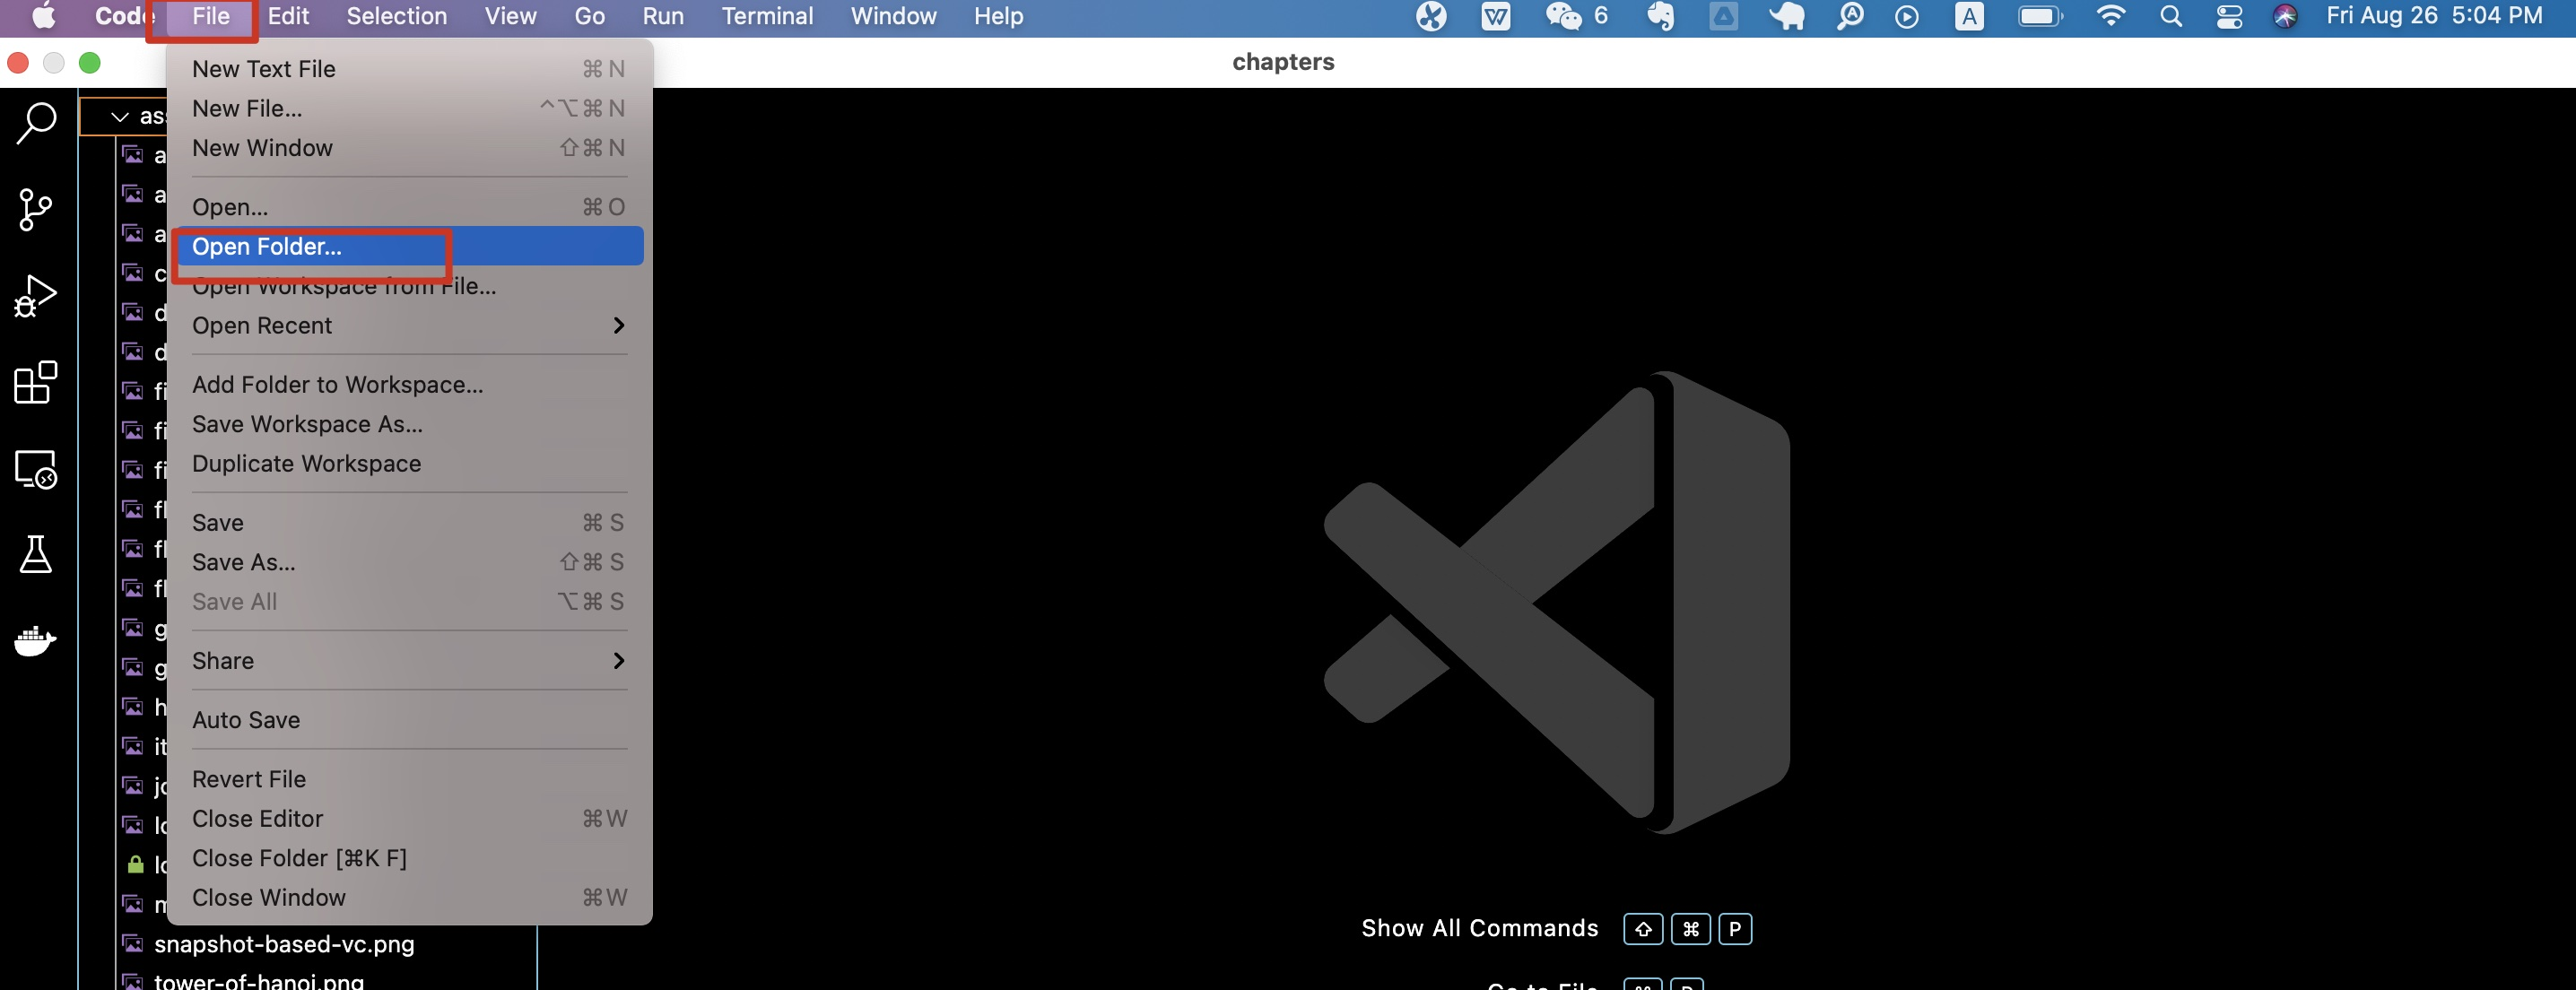
\includegraphics[width=1.3\linewidth]{assets/07-openfile-vscode.jpg}
  \caption{VS Code navigator.}
  \label{fig:vscode-navigator}
\end{marginfigure}

\begin{marginfigure}%
  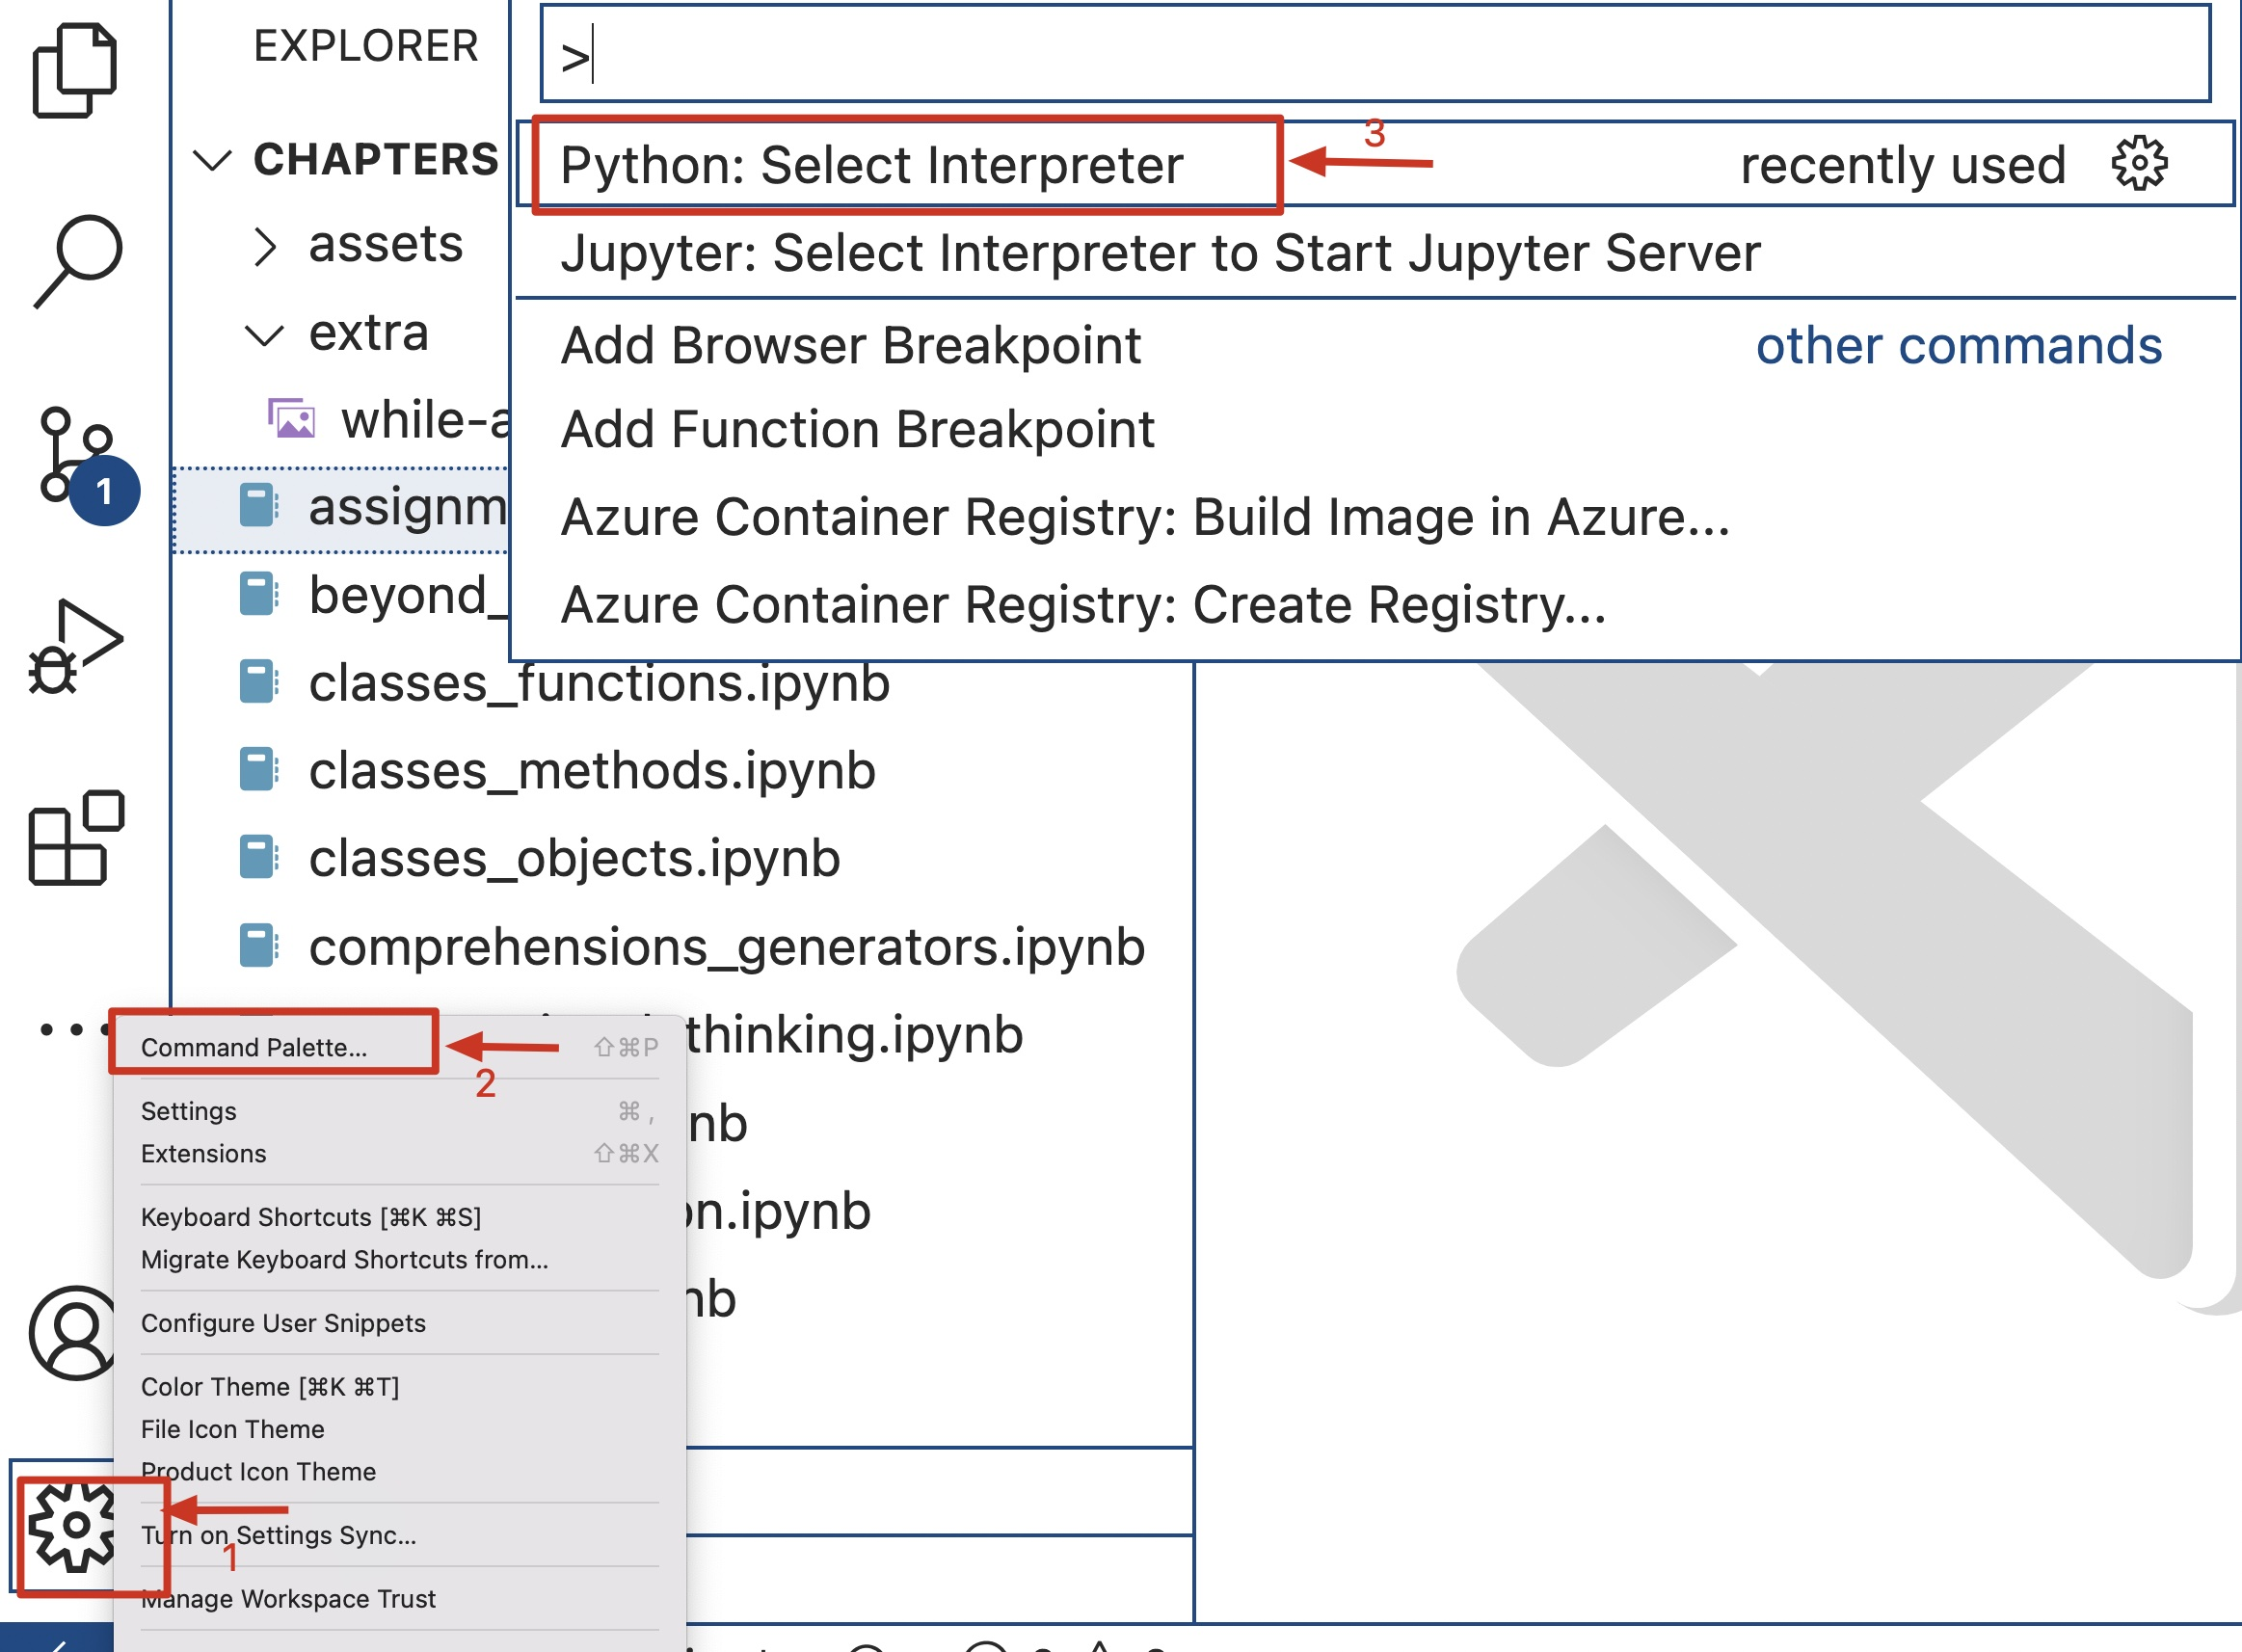
\includegraphics[width=1.3\linewidth]{assets/08-choose-env-vscode.jpg}
  \caption{Choose environment in VS Code.}
  \label{fig:environment-vscode}
\end{marginfigure}







\section{Additional Notes}
\label{additional-notes}



\subsection{Notes on Versions}\label{notes-on-versions}

\begin{itemize}
	\item Using an older version than \textbf{Python 3.8}, in particular any version of Python 2, will be problematic, because it lacks support for some important features.
	\item Using an older version than \textbf{Jupyter 6.0} will be problematic, because it lacks support for some important features.
	\item Using an older version than \textbf{Anaconda 2021-05} will be problematic, because it has a different set of libraries.
	\item Using newer versions should not be an issue, but we cannot guarantee that you won't experience issues. Do keep in mind that some features may not work as expected.
\end{itemize}

\subsection{Notes on Updating}\label{notes-on-updating}

\begin{itemize}
	\item Unless we specifically indicate otherwise, it is recommended to not update your installation.
	\item Stick with the installed version of Anaconda, Jupyter, Python, and additional libraries.
	\item We advise against updating individual parts of your installation. It is all too easy to end up with a combination that does not work satisfactorily.
\end{itemize}

\begin{center}\rule{\linewidth}{0.5pt}\end{center}


\section{Uninstalling}\label{uninstalling}

To uninstall Anaconda, please follow the guidelines provided
\href{https://docs.anaconda.com/anaconda/install/uninstall}{here}.

    \begin{center}\rule{\linewidth}{0.5pt}\end{center}


%\section{(End of Notebook)}\label{end-of-notebook}

\copyright~ Mauricio Verano Merino. 2022-2023. \textbf{VU Amsterdam - TU/e}


\end{document}
